In this report, we will explain what the Level Set method is and what its applications are. Furthermore, we will provide code examples of how to implement the mathematical formulas needed to create a Level Set framework. 

The Level Set method is a numerical technique used to track or transform surfaces in $d$ dimensions. The surfaces are tracked by solving a partial differential equation dependant on a time factor. 

The level set at its most simple representation is a static datastructure. It can be represented as a topographic map indicating heights in a region, displayed in figure \vref{introduction:fig:hoejdekort} or it can be seen as a meteorological map, displaying weather data like pressure.

\image{hoejdekort.png}{0.25}{A topographic map indicating heights in the vermont region.}{introduction:fig:hoejdekort}


\subsection{Cartesian grid}
\begin{comment}
  Finite memory -> descritization of plane -> cartesian grid is used.
\end{comment}

Since a computer has finite memory we need to come up with a way to store our representation. A simple way to do this that scale in the number of dimensions is to partition the region into a grid where each square is of equal size.

\begin{figure}[htb]
  \centering
  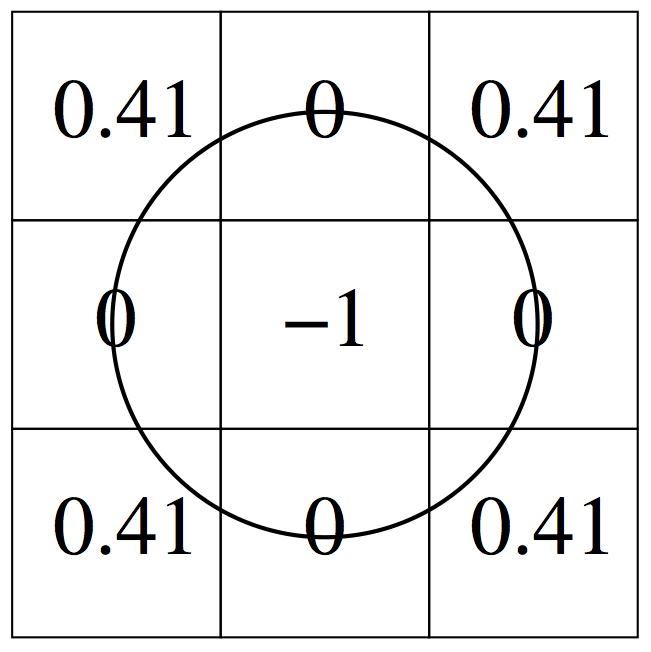
\includegraphics[scale=0.3]{imgs/cartesiangrid.png}
  \todoPtx[inline]{Lav vector version hvor der står $\sqrt{2}-1$}
  \caption{Borrowed from \cit{JLTGK}. A circle, descritized into a cartesian grid. The value in each cell is the $\phi$ value described in this chapter.}
  \label{introduction:fig:cartesiangrid}
\end{figure}

In figure \vref{introduction:fig:cartesiangrid}, we see how a plane has been descritized into a cartesian grid, showing a circle and the values of $\phi$.

\subsection{Signed distance function -  $\phi$}

We use an implicit representation of the surface. The Level Set method can use implicit functions which means that the function is defined in the entire plane and not only on the object.

The function $\phi(x,y)$ is a signed distance function in all of
$\mathbb{R}^{n}$, in our case $\mathbb{R}^{2}$. A signed distance
function $\phi$ is a function that given a point on the plane, returns
the distance to the surface. We have that $\phi(x,y) > 0$ if we are
outside the object and $\phi(x,y) < 0$ when we are inside the object.
And last, when $\phi(x,y) = 0$ we are on the interface or iso-surface. 
The iso-surface separates the inside and outside.  Besides indicating
whether we are inside or outside an object, it also indicates how far
we are from the closest point on the iso-surface which is quite
handy. For a picture of the above, see figure
\vref{introduction:fig:implicitfunction}.

\image{phi.png}{0.3}{The figure is borrowed from \cit{osher2002level}. A implicit function, defined in all of $\mathbb{R}^{2}$. We see that when we are inside the object then $\phi$ is less than zero, larger when we are outside and zero on the interface.}{introduction:fig:implicitfunction}

%% Example - Circle

\subsubsection{Example}

A simple example is to consider a circle and its equation:
\begin{equation*}
  x^{2} + y^{2} = r^{2}
\end{equation*}

It is defined in all points in $\mathbb{R}^{2}$ and is an example of an implicit function. Given a specific radius $r$, the equation of a circle defines an isocontour. If $r = 5$, then the isovalue is $c = 5^{2} = 25$. For all the points $(x,y)$ that evaluate to 25 gives us the isosurface. If the value is smaller then it is inside the surface, and outside when the value is greater. See figure \vref{introduction:fig:cartesiangrid}.

%% formulas

\begin{comment}

\subsection{Solving the Level Set}\label{sec:intro:solve}

When solving our level set, for each iteration we solve a partial differential equation in all points $(x,y) | x,y \in \mathbb{R}^{2}$. If we want to move the interface in the normal direction we solve the following equation:

\begin{equation}
\label{introduction:eq:levelsetndirection}
  \phi_{t} + a|\nabla \phi| = 0
\end{equation}\label{eq:normMove}

where $\nabla \phi = (\dfrac{\partial \phi}{\partial x}, \dfrac{\partial \phi}{\partial y})$  and $a$ can be of either sign. 

When $a > 0$ the interface moves in the normal direction and when $a < 0$ it moves in the opposite direction of the normal.

\end{comment}

\subsection{Applications}

The advantages are that since we discretize the surface into a cartesian grid, we can do numerical computations without having to parameterize the objects. Another advantage is that the level set method makes it easy to work on geometry that change topology over time.


%% applications.
So why do we want to use the level set method? A simple example is to consider an object that splits in two or two objects merging into one. If we did not use the level set method, we would have to explicitely represent the two new objects, where in the level set case we get this for free do to the implicit representation.

% lidt flere anvendelsesmuligheder (lysberegninger her!)

\newpage

\subsection{Outline of the report}\todoPtx{Denne er på en side for sige selv, så vref ikke crasher}

In chapter \vref{chap:sdf}, we give an in depth look on the signed distance function, describe what kinds of mathematical operations we have in our toolbox and describe the important reinitialize function, section \vref{sec:reinitialize}.

In chapter \vref{chap:extensions}, we look at extension that can be made to the basic level set implementation that we have done. In section \vref{sec:segmentation}, we look at how to implement segmentation algorithms which can be used in mediacal imaging. In section \vref{sec:fluid}, we implement a fluid solver for computer graphics using the level set method. And finally, in section \vref{sec:imagereconstruction} \todoHave{Skal CPVC's afsnit være med i den endelige rapport? (have)} we use the level set to do computations on images.



%%% Local Variables: 
%%% mode: latex
%%% TeX-master: "../master.tex"
%%% End: 

